{ \color{red} This section resume the Chapters 1-5 (excluding Sections 3.3 and 3.4), 6, 7 (Sections 7.1, 7.2 and 7.3) of \emph{An Introductory Time Series with R} }

\hl{A mettre dans la bio: Cowpertwait, P. and Metcalfe, A., Introductory Time Series with R, Springer, 2009.}

\paragraph{Trend}
In general, a systematic change in a time series that does not appear to be periodic is known as a trend.

\paragraph{Seasonal Variation}
A repeating pattern within any fixed period.

\paragraph{Notation}
We represent a time series of length n by ${x_t : t = 1,...,n} = {x_1, x_2, ..., x_n}$

\paragraph{Forecast}
A forecast $\hat{x}_{t+k|t}$ is a predicted future value, and the number of time steps into the future is the \textbf{lead time (k)}

\section{Base Models}

\paragraph{Additive Decomposition}
The additive decomposition model is given by
\[ x_t = m_t + s_t + z_t \]
where $t$ is the time, $x_t$ the observed series, $m_t$ the trend, $s_t$ the seasonal effect and $z_t$ the error term.

\paragraph{Multiplication Model}
If the seasonal effect tends to increase as the trend inscrease, we use a multiplication model define as
\[ x_t = m_t \cdot s_t + z_t \]
where $t$ is the time, $x_t$ the observed series, $m_t$ the trend, $s_t$ the seasonal effect and $z_t$ the error term.

\subsection{Estimating Trends}

\paragraph{Centered Moving Average}
A moving average is an average of a specified number of time series values around each value in the time series, with the exception of the first few and last few terms.
The length of the moving average is chosen to average out the seasonal effects, which can be estimated
\[ \hat{m}_t = \frac{0.5m_{t-k} + m_{t-k-1} + ... + m_t + ... + m_{t+k-1} + 0.5m_{t+k}}{2k} \]

\subsection{Estimating Seasonal Effect}

\paragraph{Additive Effect}
An estimate of the monthly additive effect ($s_t$) at time t is define by
\[ \hat{s}_t = x_t - \hat{m}_t \]
It is usual to adjust those estimate in order that the sum of one period of the time serie equal zero. Let $c$ be that adjustment in order to solve this expression.
\[ \sum (s_t + c) = 0 \]

\paragraph{Multiplicative Effect}
An estimate of the monthly multiplicative effect ($s_t$) at time t is define by
\[ \hat{s}_t = \frac{x_t}{\hat{m}_t} \]
And we found the ajustment $c$ in order to solve this expression.
\[ \sum \frac{(\hat{s}_t + c)}{n} = 1 \] 

\begin{figure}[!ht]
    \centering 
    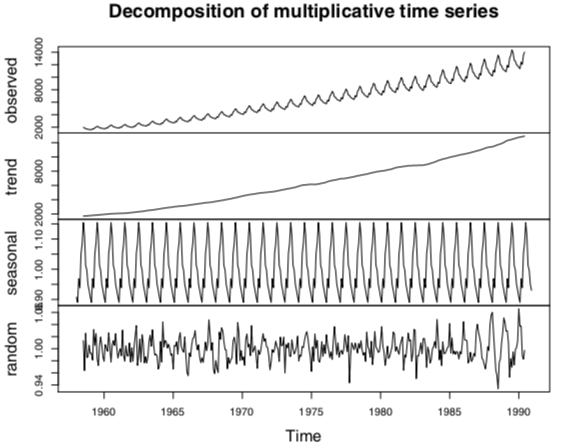
\includegraphics[scale=0.6]{src/SerieChronologique/DecompositionMultiTimeSerie.png}
    \caption{In this example, the multiplicative model would seem more appropriate than the additive model because the variance of the original series and trend increase with time} 
\end{figure}

\subsection{Smoothing Procedure}
Smoothing procedures can, and usually do, use points before and after the time at which the smoothed estimate is to be calculated. A consequence is that the smoothed series will have some points missing at the beginning and the end unless the smoothing algorithm is adapted for the end points.
\begin{itemize}
    \item[Ex.1] The centering moving average is an exemple of a \emph{smoothing} procedure. 
    \item[Ex.2] The \emph{loess} technique is also a \emph{smoothing} that use a locally weighted regression.

\end{itemize}

\section{Correlation}

\paragraph{Mean Function}
The mean function is, in general, a function of t and it define as 
\[\mu(t) = \esp{x_t} \]

\paragraph{Sample Mean}
The sample mains is define as
\[ \bar{x} = \sum \frac{x_i}{n} \]

\paragraph{Variance Function}
The variance function of a time series model that is stationary in the mean is
\[ \sigma^2(t) = \esp{(x_t - \mu^2)} \]

\paragraph{Sample Variance}
If the model is stationary in the variance, we can estimate the variance with the sample variance define as
\[ \variance{x} = \frac{\sum (x_t - \bar{x}}{n-1} \]

\paragraph{Stationarity}
If the mean function is constant, we say that the time series model is stationary in the mean. The time serie can also be stationary in the variance, if the variance function is constant $\sigma^2$.

\paragraph{Ergodic Serie}
A time series model that is stationary in the mean is ergodic in the mean if the time average for a single time series tends to the ensemble mean as the length of the time series increases.
\[ \lim_{n \to \infty} \bar{x} = \mu \]

\paragraph{Covariance}
The covariance measure the \emph{linear association} between two random variables. The covariance is define as
\[ \gamma(x,y) = \esp{(x - \mu_x)(y - \mu_y)} \]

\paragraph{Sample Covariance}
We can estimate the covariance with the sample covariance define as
\[ \covar{x, y} = \sum \frac{(x_i - \bar{x})(y_i - \bar{y})}{n-1} \]

\paragraph{Correlation}
Correlation is a dimensionless measure of the linear association between a pair of variables (x,y) and is obtained by standardising the covariance.
\[ \rho(x, y) = \frac{\esp{(x-\mu_x)(y-\mu_y)}}{\sigma_x \sigma_y} = \frac{\gamma(x,y)}{\sigma_x \sigma_y} \]
 
\paragraph{Sample Correlation}
We can estimate the covariance with the sample covariance define as
\[ \mathrm{Cor}(x, y) = \frac{\covar{x, y}}{\mathrm{sd}(x)\mathrm{sd}(y)} \]

\paragraph{Autocovariance (acvf)}
If a time series model is second-order stationary, we can define an autocovariance function (acvf), $\gamma_k$ , as a function of the lag $k$.
\[ \gamma_k = \esp{(x_t-\mu)(x_{t+k}-\mu)} \]

\paragraph{Sample Autocovariance}
The acvf function can be estimated by
\[ c_k = \frac{1}{n} \sum_{t=1}^{n-k} (x_t - \bar{x})(x_{t+k} - \bar{x}) \]

\begin{note}
The sample autocovariance at lag 0, $c_0$, is the variance calculated with a denominator $n$. 
\end{note}

\paragraph{Autocorrelation (acf)}
The lag $k$ autocorrelaton function (acf), $\rho_k$, is defined by
\[ \rho_k = \frac{\gamma_k}{\sigma^2} \]
where $\rho_0 = 1$

\paragraph{Sample Autocorrelation}
The acf function can be estimated by
\[ r_k = \frac{c_k}{c_0} \]

\paragraph{Second-order Stationary}
Suppose a the time serie that is stationary in the mean and the variance. Then, the time serie model is second-order stationary if the correlation between variable depends only on the number of time steps separating them.


\subsection{The Correlogram}
The correlogram is plot of $r_k$ against k. The main use of the correlogram is to detect autocorrelations in the time series after we have removed an estimate of the trend and seasonal variation.

\begin{itemize}
    \item[\textbullet] The x-axis gives the lag ($k$) and the y-axis gives the autocorrelation ($\rho_k$) at each lag. The unit of lag is the sampling interval. Correlation is dimensionless, so there is no unit for the y-axis.
    \item[\textbullet] The dotted lines on the correlogram are drawn at 
        \[ -\frac{1}{n} \pm \frac{2}{\sqrt{n}} \]
    \item[] If the sample acf($r_k$) falls outside these line, we have evidence against the null hypothesis that $p_k = 0$ at the 5\% level.
    \item[\textbullet] The lag at 0 is always.
\end{itemize}

\begin{figure}[!ht]
    \centering 
    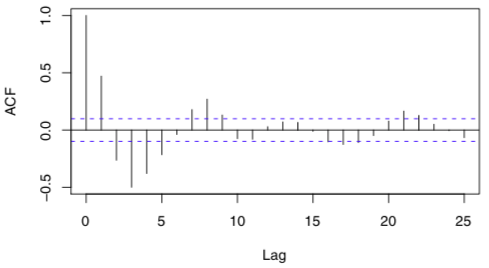
\includegraphics[scale=0.7]{src/SerieChronologique/Correlogram.png}
    \caption{Correlogram}
\end{figure}


\subsection{Covariance of sums of random variables}
Let $x_1, x_2,...,x_n$ and $y_1, y_2,..., y_m$ be random variables. Then 
\[ \covar{\sum_{i=1}^{n} x_i, \sum_{j=1}^{m}} y_j = \sum_{i=1}^{n} \sum_{j=1}^{m} \covar{x_i, y_i} \]
The result tells us that the covariance of two sums of variables is the sum of all possible covariance pairs of the variables.

\section{Forecasting Strategies}

\subsection{Relationships of different time serie}

\paragraph{Cross-covariance (ccvf)}
The cross-correlation (ccvf) between two time series is define as
\[ \gamma_k(x, y) = \esp{(x_{t+k} - \mu_x)(y_t - \mu_y)} \]

\begin{note}
    This is not a symmetric relationship, and the variable $x$ is lagging variable $y$ by $k$.
    \[\gamma_k(x, y) = \gamma_{-k}(y, x) \]
\end{note}

\paragraph{Sample Cross-covariance}
The ccvf function can be estimed by
\[ c_k(x, y) = \frac{1}{n} \sum_{t=1}^{n-k} (x_{t+k} - \bar{x})(y_k - \bar{y}) \]

\paragraph{Cross-correlation (ccf)}
The cross-correlation (ccf) between two time serie is define as 
\[ /rho_k(x, y) = \frac{\gamma_k(x, y)}{\sigma_x\sigma_y} \]

\begin{note}
    This is not a symmetric relationship, and the variable $x$ is lagging variable $y$ by $k$.
    \[\rho(x, y) = \rho_{-k}(y, x) \]
\end{note}

\paragraph{Sample Cross-correlation}
The ccf function can be estimed by
\[ r_k(x, y) = \frac{c_k(x, y)}{\sqrt{c_0(x, x) x_0(y, y)}} \]

\section{Basic Stochastic Models}

We may consider a \textbf{trend} to be \textbf{stochastic} when it shows inexplicable changes in direction. Those type of trend can be simulated by the models of this section.

\subsection{White Noise}

\paragraph{Residual Error}
A residual error is the difference between the observed value and the model predicted value at time t. Then the residual error, $x_t$, is defined by
\[ x_t = y_t - \hat{y}_t \]
where $y_t$ is the observed value and $\hat{y_t}$ the predicted value.

As the residual errors occur in time, they form a time series: $x_1, x_2,..., x_n$.

\paragraph{Definition} 
A white noise is a time serie $\{w_t : t = 1,2,...,n\}$ where each term is independent and with a constant variance $\sigma^2$.
\[ w_t \sim \mathrm{N}(0, \sigma^2) \]

\begin{figure}[!ht]
    \centering
    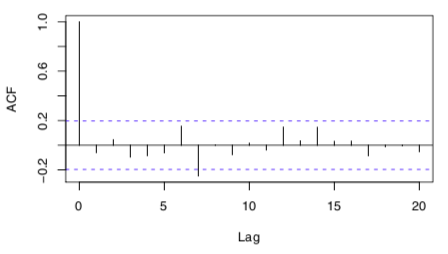
\includegraphics[scale=0.7]{src/SerieChronologique/WhiteNoise-Correlogram.png}
    \caption{Correlogram of a simulated white noise series. The underlying autocorre- lations are all zero (except at lag 0); the statistically significant value at lag 7 is due to sampling variation.}
\end{figure}

\subsection{Random Walks}

\paragraph{Definition}
Let $\{x_t\}$ be a time series. Then $\{x_t\}$ is a random walk if 
\[ x_t = x_{t-1} + w_t \]
where $\{w_t\}$ is a white noise.

\paragraph{Backward Operator}
The backward operator(or lag operator)  $\mathbf{B}$ is defined by
\[ \mathbf{B}^n = x_{t-n} \]

\paragraph{Second-order Properties}
The covariance is in function of time, so a random walk is non-stationary. This model is only suitable for short term predictions.
\begin{align*}
        \hspace*{1cm}
      \mu(t) &= 0 \\
      \sigma^2(t) &= t\sigma_w^2 \\
      \gamma_k(t) &= t\sigma_w^2 \\
      \rho_k(t) &= \frac{1}{\sqrt{1 + \frac{k}{t}}}
\end{align*} 

\paragraph{The Difference Operator}
The defference operator is defined by
\[ \nabla x_t = x_t - x_{t-1} \] 
We can also expresse it with the Backward operator
\[ \nabla^n x_t  = (1 - \mathbf{B})^n x_t \]
\begin{note}
Differencing adjacent terms of a series can transform a non-stationary series to a stationary series.
    \[ x_t - x_{t-1} = w_t \]
Here differencing two non-stationary random walk give a stationary white noise.
\end{note}

\begin{figure}[!ht]
    \centering
    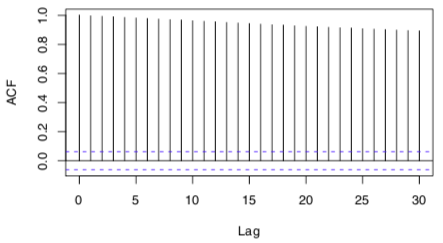
\includegraphics[scale=0.7]{src/SerieChronologique/RandomWalk-Correlogram.png}
    \caption{The correlogram for the simulated random walk. A gradual decay from a high serial correlation is a notable feature of a random walk series.}
\end{figure}

\paragraph{Random Walk with Drift}
A Random walk with drif is a random walk with a mean. it defined as
\[ x_t = \delta + x_{x-1} + w_t \] 

\subsection{Autoregressive Models}

\paragraph{Definition}
The series $\{xt\}$ is an autoregressive process of order p, abbreviated to $\mathrm{AR(p)}$, if
\[ x_t = \alpha_1 x_{t-1} + \alpha_2 x_{x-2} + ... + \alpha_p x_{t-p} + w_t \] 
where $\alpha_i$ are the model parameters with $\alpha_p \neq 0$.

The following points should be noted:
\begin{itemize} 
    \item[\textbullet] The random walk is a special case of $\mathrm{AR(1)}$ with $\alpha_1 = 1$.
    \item[\textbullet] The model is a regression of $x_t$ on past terms from the same series, that where the name \emph{autoregressive} come.
    \item[\textbullet] A prediction at time $t$ is given by
        \[ \hat{x}_t = x_t = \alpha_1 x_{t-1} + \alpha_2 x_{x-2} + ... + \alpha_p x_{t-p} \]
    \item[\textbullet] The model parameters can be estimated by minimising the sum of squared errores.
\end{itemize}

\paragraph{Stationary and non-stationary AR processes}
We can expressed a AR model as a polynomial of order p in terms of the backward shift operator
\[ \theta_p(\mathrm{B})x_t = (1 - \alpha_1\mathrm{B} - \alpha_2 \mathrm{B}^2 - ... - \alpha_p \mathrm{B}^p)x_t = w_t \]
Then a AR model is stationary if all root of $\theta_p(\mathrm{B})$ exceed one in absolute values. In other word if 
\begin{center}
if all $|\mathrm{B_i}| > 1$ then the model is stationary \\
otherwise, the model is non-stationary
\end{center}

\paragraph{Second-order properties of an AR(1) model}
    \begin{align*}
      \mu_k &= 0 \\  
      \gamma_k &= \frac{\alpha^k \sigma_w^2}{1 - \alpha^2} \\
      \rho &= \alpha^k
\end{align*}

\begin{figure}[!ht]
    \centering
    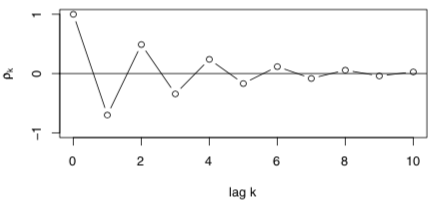
\includegraphics[scale=0.7]{src/SerieChronologique/AR-Correlogram.png}
    \caption{For an AR model, the correlograms decays to zero. The correlogram decays to zero more rapidly for small $\alpha$.}
\end{figure}

\paragraph{Partial Autocorrelation}
An AR(p) process has a correlogram of partial autocorrelation $\alpha_k$ that is zero after lag p.

\section{Regression}

When we have some plausible physical explanation for a \textbf{trend} we will usually wish to model it in some \textbf{deterministic} manner. Therefore, the model of this section can be used.
\\
\\
The difference with \textbf{deterministics trend} is the when we make short term forecast, we assume that the trend will change slowly.
\\
\\
Time series regression usually differs from a standart regression analysis because the residual form a time serie and therefore tend to be serially correlated. When this correlation is possitive, the estimated standard errors of the parameter estimates, read from the computer output of a standard re- gression analysis, will tend to be less than their true value.

\subsection{Linear Models}

\paragraph{Definition}
A model for a time series $\{ x_t : t = 1,...,n\}$ is linear if it can be expressed as
\[ x_t = \alpha_0 + \alpha_1 u_{1,t} + \alpha_2 u_{2,t} + ... + \alpha_m u_{m,t} + z_t \]
where $u_{i,t}$ is the value of the i\up{th} explanatory variable, $\alpha_i$ the estimated model parameters, $z_t$ the error at time $t$.

An example of a linear model is the pth-order polynomial function of t:
\[ x_t = \alpha_0 + \alpha_1 t + \alpha_2 t^2 + ... + \alpha_p t^p + z_t \]

\begin{note} 
    Note that the errors form a time series $\{z_t\}$, with mean 0, that does not have to be Gaussian or white noise.
\end{note} 

\paragraph{Stationarity}
Linear models for time series are non-stationary when they include functions of time.

Differencing can remove both stochastic and deterministic trends from time series. Then for a polynomial of roder $m$, the mth-order differencing is required to remove the trend.
\paragraph{Autocorrelation variance estimation of the sample mean}
Let $\{x_t : t = 1,..., n\}$ be a stationary time serie with mean $\mu$, variance $\sigma^2$ and autocovariance $\covar{x_t, x_{t+k}}$. Then the variance of the sample mean is given by
\[ \variance{\bar{x}} = \frac{\sigma^2}{n} \left[ 1 + 2 \sum_{k=1}^{n-1} (1 - \frac{k}{n}) \rho_k \right] \] 

\paragraph{Generalised least squares}
A fitting procedure known as generalised least squares (GLS) can be used to provide better estimates of the standard errors of the regression parameters to account for the autocorrelation in the residual series.

\subsection{Linear Models with Seasonal Variables}

\paragraph{Additive Seasonal Indicator Variables}
To include seasonal effect, we change the constant $\alpha_o$ depending on the season. Let $s$ be the time serie measured (Ex. for monthly time serie, $s=12$). Then for each $s$, we fit a constant term.
\[ x_t = s_t + m_t + z_t \]
where $s_t$ is the seasonal constant when t falls in the i\up{th} season, $m_t$ a linear model for the trend and $z_t$ the error term.

\paragraph{Harmonic Seasonal models}
The advantage of this model is that we can represente the seasonal effect with something that is smoothly. For a time series $\{x_t\}$ with $s$ season, there are $\lfloor s/2 \rfloor$ possible cycles. The harmonic model is defined by 
\[ x_t = m_t + \sum_{i=1}^{\lfloor s/2 \rfloor} \left\{ s_i \sin(\frac{2\pi it}{s}) + c_i \cos(\frac{2\pi it}{s}) \right\} + z_t \]
where $m_t$ is a trend model \textbf{that include a constant term} ($\alpha_0$) and $s_i$ and $c_i$ are unknown parameters. 

\begin{figure}[!ht]
    \centering 
    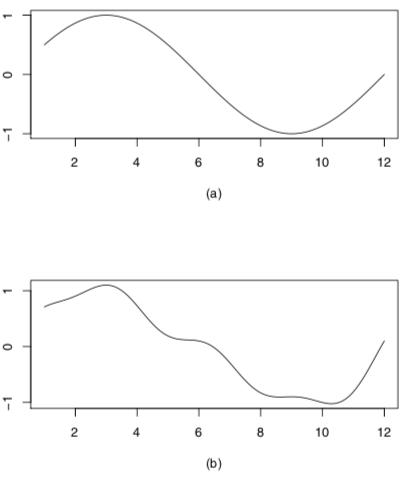
\includegraphics[scale=0.7]{src/SerieChronologique/HarmonicModel.png}
    \caption{Two possible underlying seasonal patterns for monthly series based on the harmonic model (Equation (5.10)). Plot (a) is of the first harmonic over a year and is usually too regular for most practical applications. Plot (b) is of the same wave but with a further two harmonics added. Plot (b) illustrates just one of many ways that an underlying sine wave can be perturbed to produce a less regular, but still dominant, seasonal pattern of period 12 months.}
\end{figure}

\subsection{Forecasting from regression}
When we predic a regression time series, we try to predict in the future. The problem is that the trend might change. Therefore, it is better ot think of a forecast from a regression model as an expected value conditional on past trends continuing into the future.

\paragraph{Bias Correction} 
The process of transforming the model introduce some bias in the mean. We need to apply a correction to the mean. Note that this correction doesn't need to be apply in simulation.
\[ \hat{x}_t' = \hat{x}_t * \text{Correction} \]

\subparagraph{Lognormal Correction}
\[ e^{\sigma^2 /2} \]
\subparagraph{Empirical Correction}
\[ \frac{1}{n} \sum e^{z_t} \]

\section{Stationary Models}
Sometime, the residual will be correlated in time, as this is not accounted in the fitted regression model, we need other model. 

\subsection{Strictly Stationary Series}
A time series model $\{ x_t \}$ is \emph{strictly stationry} if the joint statistical distribution $x_{t_1},...,x_{t_n}$ is the same as the joint distribution of $x_{t_1 + m},...,x_{t_n + m}$ for all $t_1, ..., t_n$ and $m$, so that the distribution is unchanged after an arbitrary time shift.

\begin{note}
    Note that strict stationarity implies that the mean and variance are constant in time and that the autocovariance $ \covar{x_t, x_s} = \gamma_k$ (i.e. only depend on the lag $k$). If a series is not strictly stationary but the mean and variance are constant in time and the autocovariance only depends on the lag, then the series is called \emph{second-order stationary}.
\end{note}
We focus on the second-order properties in this chapter, but the stochastic processes discussed are strictly stationary.
\\ 
\\
Stationarity is an idealisation that is a property of models. If we fit a stationary model to data, we assume our data are a realisation of a stationary process. So our first step in an analysis should be to check whether there is any evidence of a trend or seasonal effects and, if there is, remove them. Regression can break down a non-stationary series to a trend, seasonal components, and residual series. It is often reasonable to treat the time series of residuals as a realisation of a stationary error series. Therefore, the models in this chapter are often fitted to residual series arising from regression analyses.

\subsection{Moving average models}

\paragraph{Definition}
 moving average (MA) process of order q is a linear combination of the current white noise term and the q most recent past white noise terms and is defined by
\[ x_t = w_t + \beta_1 w_{t-1} + ... + \beta_q w_{t-q} = \phi_q(\mathrm{B}) w_t \]
where $\phi_q$ is a polynomial of order q. Because MA processes consist of a finite sum of stationary white noise terms, they are stationary and hence have a time-invariant mean and autocovariance.

\paragraph{Second-order properties}
\begin{align*}
    \mu &= 0 \\
    \sigma^2 &= \sigma_w^2 (1 + \beta_1^2 + ... + \beta_q^2) \\
    \gamma_k &= \sigma_w^2 \sum_{i=0}^{q-k} \beta_i \beta_{i+k} \\
    \rho_k &= \frac{\sum_{i=0}^{q-k} \beta_i \beta_{i+k}}{\sum_{i=0}{q} \beta_i^2 }
\end{align*}
where $\beta_0 = 1$.

\paragraph{Invertible properties}
An MA process is invertible if it can be expressed as a stationary AR($\infty$) process of infinite order without an error term.
\[ w_t = (1 - \beta \mathrm{B})^{-1} x_t = x_t + \beta x_{t-1} + \beta^2 x_{t-2} + ... \]
provided $|\beta| < 1$, which is required for convergence.

\begin{figure}[!ht]
    \centering
    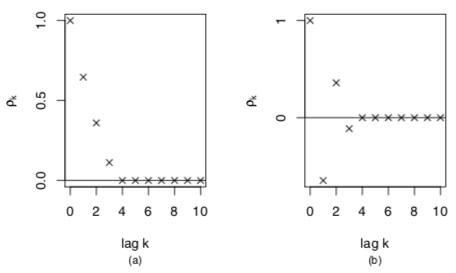
\includegraphics[scale=0.7]{src/SerieChronologique/MA-Correlogram.png}
    \caption{Plots of the autocorrelation functions for two MA(3) processes. The autocorrelation for lag $k>q$ are all zero. $(a) \beta_1 = 0.7, \beta_2 = 0.5, \beta_3 = 0.2; (b) \beta_1 = -0.7, \beta_2 = 0.5, \beta_3 = -0.2$.}
\end{figure}

\subsection{Mized Models: The ARMA process}

\paragraph{Definition}
The ARMA model is a AR(p) + MA(q) models defined as
\[ x_t = \alpha_1 x_{t-1} + \alpha_2 x_{t-2} + ... + \alpha_p x_{t-p} + w_t + \beta_1 w_{t-1} + \beta_2 w_{t-2} + ... + \beta_q w_{t-q} \]
We can also express it as 
\[ \theta_p(\mathrm{B}) x_t = \phi_q(\mathrm{B}) w_t \]
\begin{itemize}
    \item[\textbullet] The process is stationary when the roots of $\theta$ are all exceed unity in absolute value.
    \item[\textbullet] The process is invertible when the roots of $\phi$ all exceed unity in absolute value.
    \item[\textbullet] The AR(p) model is the special case ARMA(p, 0).
    \item[\textbullet] The MA(q) model is the special case ARMA(0, q).
    \item[\textbullet] \textbf{Parameter parsimony.} When fitting to data, an ARMA model will often be more parameter efficient (i.e., require fewer parameters) than a single MA or AR model.
    \item[\textbullet] \textbf{Parameter redundancy.} When $\theta$ and $\phi$ share a common factor, a stationary model can be simplified. For example, the model:
        \begin{align*}
            (1 - \frac{1}{2}B)(1 - \frac{1}{3}B)x_t &= (1 - frac{1}{2}B)w_t \\
            (1 - \frac{1}{3}B)x_t &= w_t
        \end{align*}
\end{itemize}

\paragraph{Second-order Properties}
\begin{align*}
    \sigma^2 &= \sigma_w^2 \left( 1 + \frac{(\alpha+\beta)^2}{1 - \alpha^2} \right) \\
    \gamma_0 &= \sigma_w^2 \left( \frac{1 + 2 \alpha \beta + \beta^2}{1 - \alpha^2} \right) \\
    \gamma_k &= \sigma_w^2 (\alpha + \beta)\alpha^{k-1} \left( \frac{1 + \alpha \beta}{1 - \alpha^2} \right) \\
    \rho_k &= \frac{\alpha^{k-1}(\alpha+\beta)(1+\alpha\beta)}{1 + \alpha\beta + \beta^2} = \alpha \rho_{k-1}
\end{align*}

\section{Non-stationary Models}

\subsection{Differencing}
Differencing a serie $\{x_t\}$ can remove trends, whether these trend are stochastic, as in a random walk, or deterministic, as in the case of a linear trend. 

\subparagraph{Differencing random walk}
\[ \nabla x_t = x_t - x_{t-1} = w_t \]
which is a stationary white noise.

\subparagraph{Differencing linear trend}
\[ \nabla x_t = x_t - x_{t-1} = b + w_t - w_{t-1} \]
which is a stationary moving average process rather than white noise.

\paragraph{Integrated Model}
A serie $\{x_t\}$ is integrated of order d, $I(d)$, if the d\up{th} difference of $\{x_t\}$ is a white noise
\[ (1 - \mathrm{B})^d x_t = w_t \]

\begin{note}
    The random walk is a special case $I(1)$
\end{note}

\subsection{Non-Seasonal ARIMA Models}

\paragraph{Definition}
A time series $\{x_t\}$ follows an ARIMA($p, d, q$) process id the d\up{th} differences of the $\{x_t\}$ series are an ARIMA($p, q$) process
\[ \theta_p(\mathrm{B}(1 - \mathrm{B})^d x_t = \phi_q(\mathrm{B}) w_t \]

In general:
\begin{itemize}
    \item[\textbullet] $\text{ARIMA}(0,d,q) \equiv \text{IMA}(d, q)$
    \item[\textbullet] $\text{ARIMA}(p,d,0) \equiv \text{ARI}(p,d)$
\end{itemize}

\subsection{Seasonal ARIMA models}
A seasonal ARIMA model uses differencing at a lag equal to the number of seasons (s) to remove additive seasonal effects. As with lag 1 differencing to remove a trend, the lag s differencing introduces a moving average term.
\\
\\
The ARIMA$(p,d,q)(P,D,Q)_s$ model can be defined as
\[ \Theta_P(\mathrm{B}^s)\theta_p(\mathrm{ B})(1 - \mathrm{B}^s)^D (1 - \mathrm{B})^d x_t = \Phi_Q(\mathrm{B}^s) \phi_q(\mathrm{B}) w_t \]

